\section{Prosedur Penelitian dan Pengembangan}


\subsection{Data Penelitian}
    
Berdasarkan studi kasus dalam skripsi ini, data yang akan digunakan dalam penelitian ini adalah data koordinat dari seluruh SMA di Kabupaten Probolinggo. Data nama-nama sekolah dikumpulkan dari \url{https://data.sekolah-kita.net}, dan data koordinat dikumpulkan melalui aplikasi Google Earth yang dapat diunduh langsug ke dalam bentuk spreadsheet. Waktu yang diperlukan peneliti untuk mengumpulkan data dari web tersebut kurang lebih sekitar satu bulan.

\subsection{Instrumen Pendukung}
\begin{enumerate}
    \item Python
    
    Dalam penelitian ini akan digunakan bahasa pemrograman python untuk mempermudah pengerjaan. Bahasa python adalah bahasa pemrograman baru di masa sekarang, karena dalam bahasa ini lebih simple dan singkat dalam membuat program \cite{syahrudin2018input}. Bahasa pemrograman ini merupakan bahasa pemrograman yang paling mudah dipelajari dari pada bahasa pemrograman yang lain. Serta dalam bahasa pemrograman ini dapat menjalankan beberapa rumus matematika di dalamnya. Selain itu bahasa Python telah digunakan secara luas, dan masuk dalam 3 besar bahasa pemrograman yang digunakan dalam beberapa tahun belakangan.
    
    \item Jupyter Notebook
    
    Jupyter Notebook adalah aplikasi web gratis yang digunakan untuk membuat dan membagikan dokumen yang memiliki kode, hasil hitungan, visualisasi, dan teks. Notebook ini juga mendukung 3 bahasa pemrograman salah satunya adalah bahasa pemrograman python. Banyak kelebihan yang disajikan dari aplikasi ini salah satunya adalah mendokumentasikan kode, dan menjalankan kode dalam setiap sel, dan visualisasi data seperti pada Gambar \ref{fig:visjupyter}.

\begin{figure}[h!]
  \centering
  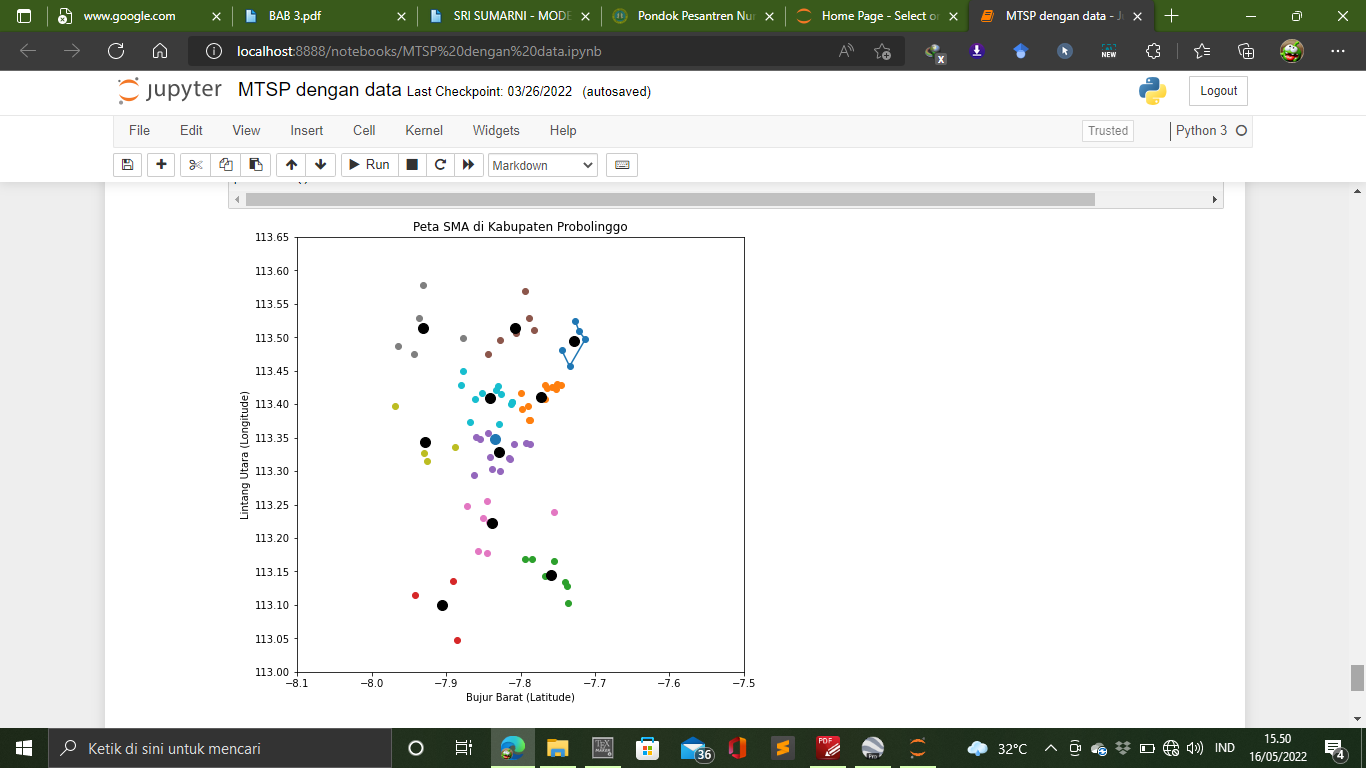
\includegraphics[width=0.8\textwidth]{visualisasi jupyter.png}
  \caption{Visualisasi data jupyter notebook}
  \label{fig:visjupyter}
\end{figure}

	\item Google Earth
	
	Google earth digunakan dalam penelitian ini untuk mengumpulkan koordinat lokasi seluruh SMA di Kabupaten Probolinggo. Aplikasi ini dapat menandai beberapa lokasi secara langsung seperti pada Gambar \ref{fig:markloc} dan mengekspor kedalam bentuk spreadsheet seperti pada Gambar \ref{fig:eksspread}. Data-data lokasi yang telah didownload ke dalam bentuk spreadsheet akan diproses menggunakan jupyter notebook.

\begin{figure}[h!]
  \centering
  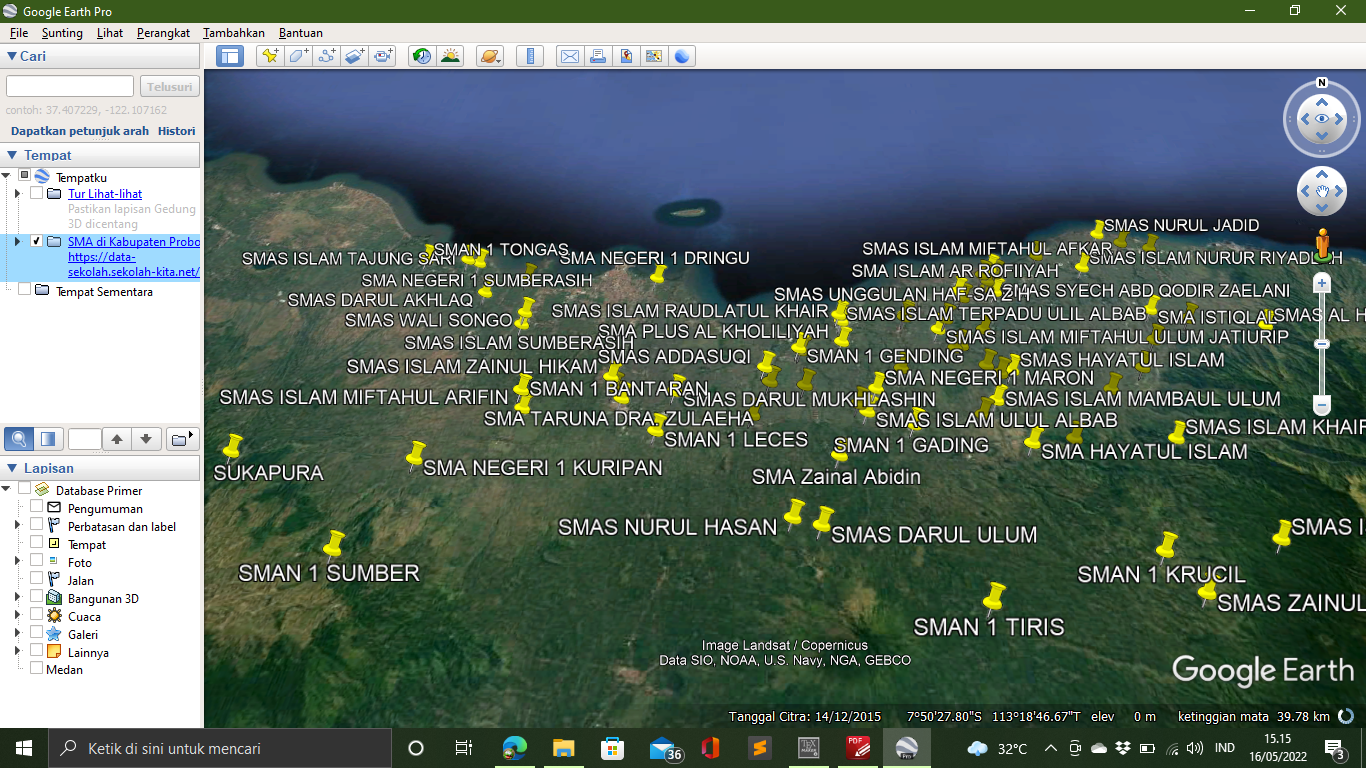
\includegraphics[width=0.8\textwidth]{google earth.png}
  \caption{Menandai lokasi pada google earth}
  \label{fig:markloc}
\end{figure}

\begin{figure}[h!]
  \centering
  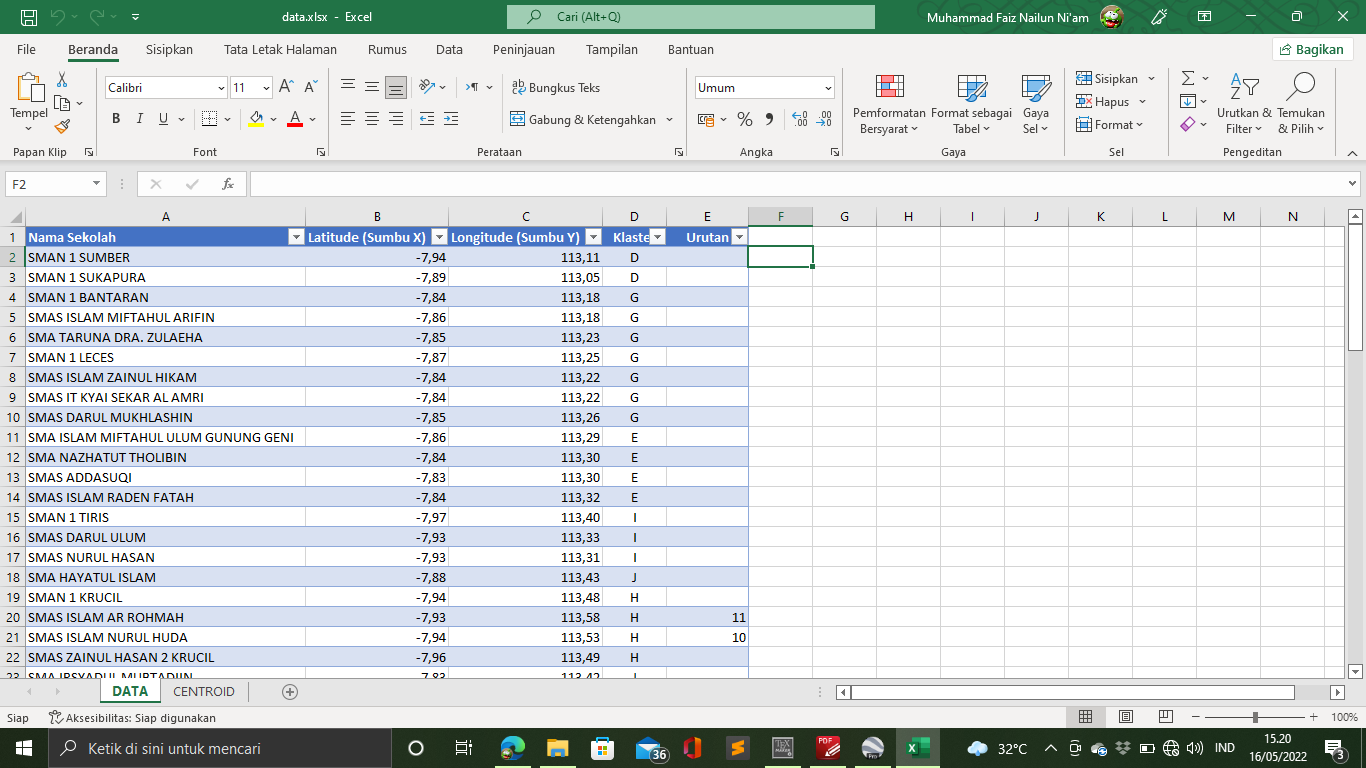
\includegraphics[width=0.8\textwidth]{ekspor spreadsheet.png}
  \caption{Mengekspor data ke bentuk spreadsheet}
  \label{fig:eksspread}
\end{figure}

\end{enumerate}

\subsection{Langkah-langkah Dalam Tahap Pengolahan Data}
\begin{enumerate}
    \item Menyiapkan data yang telah dikumpulkan sebelumnya.
    \item Selanjutnya menentukan jumlah klaster yaitu sebanyak $n$ klaster. Data yang telah dikumupulkan pada tahap ini akan dibagi menjadi beberapa klaster, metode yang digunakan algoritma \textit{k}-means.
    \item Langkah-langkah yang digunakan dalam metode \textit{k}-means adalah sebagai berikut
    \begin{enumerate}
        \item Tentukan jumlah klaster
        \item Pilih titik-titik centroid sesuai banyak klaster
        \item \label{ulang1} Hitung jarak tiap titik tujuan dengan masing-masing \textit{centroid} dengan rumus \textit{euclidean distance} seperti pada Persamaan (\ref{eq:euclidean}).
        \begin{equation}
        d_{xy}=\sqrt{\sum_{i=1}^{n}(x_i-y_i)^{2}}
        \label{eq:euclidean}
        \end{equation}
        \item Setelah seluruh titik masuk ke dalam klaster, hitung \textit{centroid} baru dengan cara menghitung rata-rata titik pada klaster tersebut. Lakukan hal yang sama pada klaster yang lain.
        \item Ulangi langkah \ref{ulang1} sampai tidak ada perubahan pada anggota klaster.
    \end{enumerate}
	
	\item Selanjutnya melakukan proses TSP pada setiap klaster yang telah dibagi, langkah-langkahnya adalah sebagai berikut.
	\begin{enumerate}
	    \item Membuat populasi awal secara random menggunakan data yang telah diklaster
	    \item \label{ulang2} Melakukan reproduksi dengan metode \textit{crosover} dengan peluang 0,95
	    \item Melakukan mutasi pada data dengan peluang 0,01
	    \item Selanjutnya seleksi dengan mode eliminasi
	    \item Menentukan nilai fitness agar mendapatkan solusi akhir yang optimal
	    \item Iterasi dilakukan dengan cara kembali ke tahapan (\ref{ulang2}) untuk generasi berikutnya sampai hasil yang dilakukan optimal atau mendekati optimal.
    \end{enumerate}
	\item Ketika proses diatas selesai dilakukan maka dihasilkanlah pembagian klaster dan rute terdekat tiap klaster menuju seluruh SMA di Kabupaten Probolinggo
	\item Mengevaluasi data yang dihasilkan
\end{enumerate}